\chapter{Análisis y diseño}
\label{cap:analisis_diseno}

En este capítulo se describe la estructura y el funcionamiento de la página web. En primer lugar, se presentan los casos de uso para mostrar qué actividades puede realizar cada usuario dentro del sistema (el alumno, el maestro y la coordinación), detallando los pasos a seguir y las reglas obligatorias que no se pueden romper. Posteriormente, se abordan el diseño de la base de datos y la organización de las pantallas.

\section{Casos de Uso de la Página Web}
\label{sec:casos_uso}

Para entender con facilidad qué tareas puede realizar cada persona dentro de la página web, a continuación se explican por separado las cuatro actividades principales. En cada una se detalla quién participa, los pasos que se siguen de inicio a fin y las reglas obligatorias que no se pueden romper para que todo funcione de forma ordenada y los alumnos no se atrasen con su tesis \parencite{sim2023technology}.

% ----------------------------------------------------------------------
% CASO DE USO 1: INICIO DE SESIÓN
% ----------------------------------------------------------------------
\subsection{Caso de Uso 1: Iniciar Sesión en la Página Web (CU01)}
\label{subsec:cu01}

En este apartado se explica cómo entran los alumnos, los maestros y el coordinador a su cuenta usando su correo de la escuela y su contraseña, para que cada quien vea únicamente la información que le corresponde.

\begin{small}
\begin{longtable}{p{3.5cm} p{11.5cm}}
\caption{Descripción del Caso de Uso 1: Iniciar Sesión.} \label{tab:cu01} \\
\toprule
\textbf{Elemento} & \textbf{Detalle descriptivo} \\
\midrule
\endfirsthead

\multicolumn{2}{c}{\tablename\ \thetable\ -- Continuación de la página anterior} \\
\toprule
\textbf{Elemento} & \textbf{Detalle descriptivo} \\
\midrule
\endhead

\bottomrule
\endfoot

\bottomrule
\endlastfoot

\textbf{Identificador} & CU01 \\ \addlinespace
\textbf{Nombre} & Iniciar sesión en la página web \\ \addlinespace
\textbf{Participantes} & Alumno, Tutor o Maestro y Coordinador. \\ \addlinespace
\textbf{Propósito} & Revisar que la persona sea quien dice ser para permitirle entrar a sus pantallas de trabajo. \\ \addlinespace
\textbf{Requisitos previos} & Que la persona tenga una cuenta registrada y activa con su correo de la escuela. \\ \addlinespace
\textbf{Pasos principales} & 
1. La persona entra a la dirección de la página web desde su navegador de internet.\par
2. La pantalla le pide escribir su correo de la escuela y su clave de acceso.\par
3. El usuario escribe sus datos y presiona el botón para entrar.\par
4. La página web revisa si los datos coinciden con la información guardada.\par
5. Si todo está correcto, la página web abre la pantalla que le toca a cada uno:\par
\quad $\bullet$ Al alumno le muestra sus tareas y entregas pendientes.\par
\quad $\bullet$ Al maestro le muestra la lista de sus alumnos asesorados.\par
\quad $\bullet$ Al coordinador le muestra el listado general de toda la escuela. \\ \addlinespace
\textbf{Caminos alternativos} & 
$\bullet$ Si el correo o la contraseña están mal escritos, la página web muestra un aviso en color rojo para que lo vuelva a intentar.\par
$\bullet$ Si la cuenta está desactivada, la página web no deja pasar al usuario y le pide acudir con la coordinación. \\ \addlinespace
\textbf{Regla obligatoria} & \textbf{Privacidad de la cuenta:} Nadie puede ver información ajena; ningún alumno podrá entrar a ver los documentos o notas de otro compañero. \\
\end{longtable}
\end{small}

Para ver de forma más clara cómo entran los usuarios a la página web, en la Figura~\ref{fig:cu01_login} se muestra el dibujo donde se aprecia la revisión de los datos y el mensaje de aviso cuando la contraseña no es correcta.

\begin{figure}[H]
    \centering
    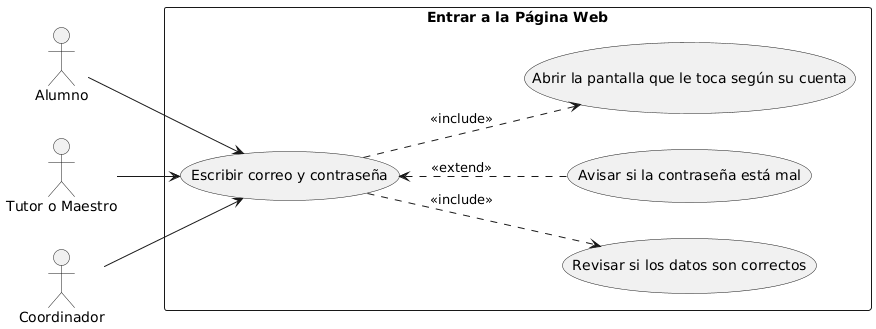
\includegraphics[width=0.88\textwidth]{assets/casos_uso/cu01_login.png}
    \caption{Diagrama del Caso de Uso 1: Iniciar Sesión en la Página Web.}
    \label{fig:cu01_login}
\end{figure}

% ----------------------------------------------------------------------
% CASO DE USO 2: REVISIÓN Y ENTREGA DE BORRADORES
% ----------------------------------------------------------------------
\subsection{Caso de Uso 2: Subir y Revisar Borradores de Tesis en PDF (CU02)}
\label{subsec:cu02}

En esta parte se muestra el camino para que el alumno entregue sus archivos de tesis, el maestro los pueda descargar para leerlos y dejar comentarios con correcciones, y la coordinación pueda ver que el trabajo siga avanzando sin perder copias viejas.

\begin{small}
\begin{longtable}{p{3.5cm} p{11.5cm}}
\caption{Descripción del Caso de Uso 2: Subida y revisión de tesis.} \label{tab:cu02} \\
\toprule
\textbf{Elemento} & \textbf{Detalle descriptivo} \\
\midrule
\endfirsthead

\multicolumn{2}{c}{\tablename\ \thetable\ -- Continuación de la página anterior} \\
\toprule
\textbf{Elemento} & \textbf{Detalle descriptivo} \\
\midrule
\endhead

\bottomrule
\endfoot

\bottomrule
\endlastfoot

\textbf{Identificador} & CU02 \\ \addlinespace
\textbf{Nombre} & Manejo y entrega de borradores de tesis \\ \addlinespace
\textbf{Participantes} & Alumno (sube el trabajo), Tutor o Maestro (descarga y revisa), Coordinador (revisa el avance general). \\ \addlinespace
\textbf{Propósito} & Guardar ordenadamente los archivos de la tesis para conservar la historia completa de cambios. \\ \addlinespace
\textbf{Requisitos previos} & Que el alumno tenga una cuenta activa y un maestro asignado en la página web. \\ \addlinespace
\textbf{Pasos principales} & 
1. El alumno entra a su apartado de entregas dentro de la página web.\par
2. Elige el archivo en su computadora, escribe una nota opcional y presiona ``Subir borrador''.\par
3. La página web revisa el archivo y le asigna un número de versión para ordenarlo (Versión 1, Versión 2, etc.).\par
4. El maestro entra a la página web y ve que su alumno subió un trabajo nuevo.\par
5. El maestro presiona el archivo para descargarlo y leerlo con calma.\par
6. En esa misma pantalla, el maestro anota sus observaciones o correcciones y las guarda.\par
7. Tanto el alumno como la coordinación pueden revisar la lista de entregas pasadas y los comentarios del maestro. \\ \addlinespace
\textbf{Caminos alternativos} & Si el estudiante intenta subir un archivo en un formato que no sea PDF (como Word o fotos), la página web lo rechaza y le pide elegir un documento en PDF. \\ \addlinespace
\textbf{Reglas obligatorias} & 
1. \textbf{Solo formato PDF:} Únicamente se aceptan archivos PDF para asegurar que las letras, tablas e imágenes no se muevan de lugar al abrirlos en otra computadora \parencite{iso32000}.\par
2. \textbf{No borrar archivos viejos:} La página web prohíbe eliminar o sobreescribir trabajos anteriores; cada entrega se guarda aparte para no perder ninguna corrección \parencite{chacon2014progit}. \\
\end{longtable}
\end{small}

En la Figura~\ref{fig:cu02_avances} se muestra el diagrama con las acciones de este apartado, donde se ve cómo el alumno sube el documento y el maestro lo descarga para responderle con sus observaciones.

\begin{figure}[H]
    \centering
    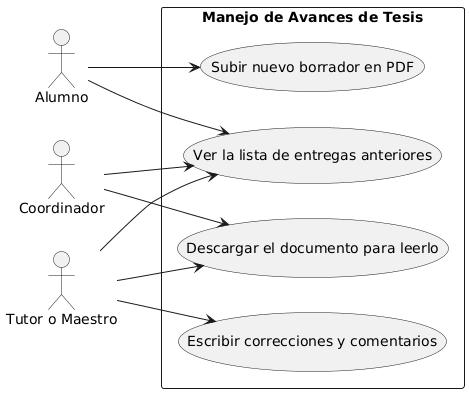
\includegraphics[width=0.72\textwidth]{assets/casos_uso/cu02_avances.png}
    \caption{Diagrama del Caso de Uso 2: Manejo de Avances de Tesis.}
    \label{fig:cu02_avances}
\end{figure}

% ----------------------------------------------------------------------
% CASO DE USO 3: REGISTRO DE MINUTAS
% ----------------------------------------------------------------------
\subsection{Caso de Uso 3: Llenar y Consultar Minutas de Asesoría (CU03)}
\label{subsec:cu03}

Aquí se explica la forma en que se guardan los acuerdos por escrito cada vez que el maestro y el alumno se juntan a revisar la tesis, evitando que las tareas se olviden con los días.

\begin{small}
\begin{longtable}{p{3.5cm} p{11.5cm}}
\caption{Descripción del Caso de Uso 3: Minutas de asesoría.} \label{tab:cu03} \\
\toprule
\textbf{Elemento} & \textbf{Detalle descriptivo} \\
\midrule
\endfirsthead

\multicolumn{2}{c}{\tablename\ \thetable\ -- Continuación de la página anterior} \\
\toprule
\textbf{Elemento} & \textbf{Detalle descriptivo} \\
\midrule
\endhead

\bottomrule
\endfoot

\bottomrule
\endlastfoot

\textbf{Identificador} & CU03 \\ \addlinespace
\textbf{Nombre} & Llenar y consultar minutas de asesoría \\ \addlinespace
\textbf{Participantes} & Tutor o Maestro (escribe la minuta), Alumno (revisa sus tareas), Coordinador (supervisa las reuniones). \\ \addlinespace
\textbf{Propósito} & Dejar un registro claro de lo que se habló en la reunión y qué tareas debe entregar cada quien para la siguiente cita. \\ \addlinespace
\textbf{Requisitos previos} & Haber terminado una reunión de asesoría (ya sea en persona o por videollamada). \\ \addlinespace
\textbf{Pasos principales} & 
1. Al terminar la reunión, el maestro entra a la sección de minutas en la página web.\par
2. Presiona el botón que dice ``Nueva minuta''.\par
3. Anota la fecha del día y un resumen corto de los temas de los que hablaron.\par
4. En la parte de compromisos, escribe las tareas pendientes, quién las va a hacer (el alumno o el maestro) y para qué fecha deben estar listas.\par
5. Presiona el botón de guardar.\par
6. La página web guarda los datos al instante.\par
7. El alumno puede entrar en cualquier momento a consultar qué tareas tiene pendientes y cuándo entregarlas. \\ \addlinespace
\textbf{Caminos alternativos} & Si el maestro intenta guardar la minuta dejando espacios en blanco o sin anotar compromisos, la página web no lo deja guardar y le avisa qué datos le faltan. \\ \addlinespace
\textbf{Regla obligatoria} & \textbf{Datos obligatorios:} Toda minuta debe llevar forzosamente la fecha de la reunión, de qué hablaron y por lo menos una tarea con fecha límite de entrega. \\
\end{longtable}
\end{small}

Para entender el proceso de forma visual, en la Figura~\ref{fig:cu03_minutas} se representa el diagrama de cómo el maestro anota los acuerdos y cómo los demás usuarios pueden consultar esa información.

\begin{figure}[H]
    \centering
    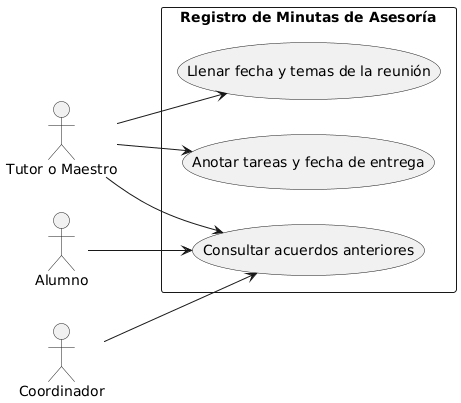
\includegraphics[width=0.68\textwidth]{assets/casos_uso/cu03_minutas.png}
    \caption{Diagrama del Caso de Uso 3: Registro de Minutas de Asesoría.}
    \label{fig:cu03_minutas}
\end{figure}

% ----------------------------------------------------------------------
% CASO DE USO 4: ALERTAS DE INACTIVIDAD
% ----------------------------------------------------------------------
\subsection{Caso de Uso 4: Avisos por Inactividad Mayor a 30 Días (CU04)}
\label{subsec:cu04}

Este caso de uso describe la función que hace la página web de contar los días sin actividad para avisar a los maestros y a la coordinación cuando un estudiante se está quedando atrás y necesita apoyo.

\begin{small}
\begin{longtable}{p{3.5cm} p{11.5cm}}
\caption{Descripción del Caso de Uso 4: Avisos de inactividad.} \label{tab:cu04} \\
\toprule
\textbf{Elemento} & \textbf{Detalle descriptivo} \\
\midrule
\endfirsthead

\multicolumn{2}{c}{\tablename\ \thetable\ -- Continuación de la página anterior} \\
\toprule
\textbf{Elemento} & \textbf{Detalle descriptivo} \\
\midrule
\endhead

\bottomrule
\endfoot

\bottomrule
\endlastfoot

\textbf{Identificador} & CU04 \\ \addlinespace
\textbf{Nombre} & Detección y aviso de inactividad mayor a 30 días \\ \addlinespace
\textbf{Participantes} & Página Web (reloj automático), Tutor o Maestro (cuida a sus alumnos), Coordinador (revisa a todos los alumnos). \\ \addlinespace
\textbf{Propósito} & Avisar a tiempo si un alumno lleva mucho tiempo sin comunicarse o sin entregar avances, para ayudarlo antes de que deje la tesis \parencite{lando2025digital}. \\ \addlinespace
\textbf{Requisitos previos} & Que los alumnos estén registrados y tengan la fecha de su último trabajo o de su última reunión. \\ \addlinespace
\textbf{Pasos principales} & 
1. La página web compara la fecha de hoy con el último día en que el estudiante subió un archivo o tuvo una reunión.\par
2. La página web cuenta cuántos días han pasado sin registrar nada nuevo.\par
3. Si la cuenta pasa de los 30 días, la página web le pone una marca de alerta al expediente del estudiante.\par
4. Cuando el maestro abre su lista de tesistas, ve un aviso junto al nombre del alumno atrasado.\par
5. Cuando el coordinador abre su pantalla, ve una lista con todos los alumnos que tienen alerta para llamarlos o mandarles un mensaje a tiempo. \\ \addlinespace
\textbf{Caminos alternativos} & En cuanto el alumno vuelve a subir un trabajo en PDF o el maestro registra una nueva minuta, el contador de días se regresa a cero y el aviso de alerta se apaga automáticamente. \\ \addlinespace
\textbf{Regla obligatoria} & \textbf{Tiempo límite de 30 días:} El aviso se enciende únicamente cuando el alumno acumula más de 30 días seguidos sin entregar ningún trabajo y sin registrar minutas de asesoría. \\
\end{longtable}
\end{small}

De forma gráfica, en la Figura~\ref{fig:cu04_atrasos} se muestra cómo el reloj de la página web cuenta los días y activa la lista de alertas para que los maestros y la coordinación puedan intervenir a tiempo.

\begin{figure}[H]
    \centering
    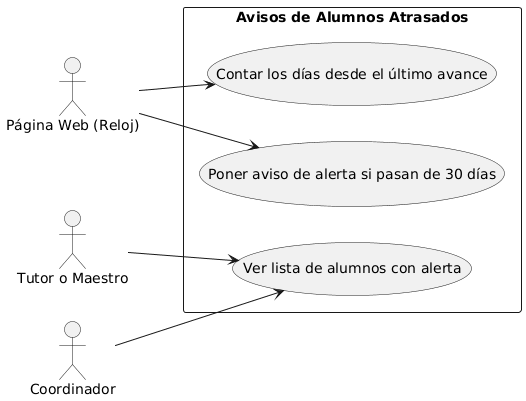
\includegraphics[width=0.68\textwidth]{assets/casos_uso/cu04_atrasos.png}
    \caption{Diagrama del Caso de Uso 4: Avisos de Alumnos Atrasados.}
    \label{fig:cu04_atrasos}
\end{figure}
\section{Diseño de la Base de Datos}
\label{sec:diseno_bd}

En este apartado se explica cómo se guarda y se organiza la información dentro de la página web usando una base de datos relacional \parencite{silberschatz2014}. Toda la información se reparte en tablas conectadas entre sí para que nada se pierda ni se revuelva, asegurando que las cuentas funcionen bien, los archivos en PDF se guarden por versiones sin borrar nada viejo, las reuniones queden registradas con sus tareas y el sistema avise si alguien pasa más de un mes sin trabajar \parencite{sim2023technology}.

\subsection{Descripción del Proyecto y Elementos de la Base de Datos}
\label{subsec:descripcion_bd}

Para entender el diagrama del sistema, la información se organiza en tres cosas muy sencillas: las tablas principales que representan a los elementos del sistema (rectángulos), los datos específicos que guarda cada una (óvalos o bolitas) y las conexiones que explican cómo se relacionan entre sí (rombos) \parencite{silberschatz2014}.

\subsubsection{Tablas y qué datos guarda cada una}

La base de datos empieza con la tabla llamada \textit{usuario}, que sirve para controlar el acceso de todas las personas a la página web. Esta tabla utiliza como dato principal el \underline{id\_usuario}, que es un número único para cada cuenta que no se repite. Además, guarda datos básicos como el \textit{correo\_institucional} para iniciar sesión, la \textit{contrasena}, la \textit{fecha\_registro} y la casilla de \textit{cuenta\_activa} para saber si la persona puede entrar o está dada de baja. El nombre de la persona se guarda en un dato llamado \textit{nombre\_completo}, el cual se divide en primer nombre, segundo nombre, apellido paterno y apellido materno para que sea fácil ordenar las listas por orden alfabético. También incluye el dato de \textit{telefono}, que se dibuja con doble óvalo porque una persona puede registrar más de un número para que la localicen. Como no todos hacen lo mismo en la página web, esta cuenta general se divide en tres tipos de usuario: el \textit{alumno}, que guarda su matrícula escolar; el \textit{asesor}, que guarda su número de maestro y su grado de estudios; y el \textit{coordinador}, que guarda el número de su oficina y su teléfono de atención.

La siguiente tabla es \textit{proyecto\_tesis}, que funciona como el expediente principal del trabajo de investigación. Tiene su propio identificador llamado \underline{id\_proyecto} y guarda datos como el \textit{titulo\_tesis}, el tema o \textit{linea\_investigacion}, la \textit{fecha\_inicio}, la \textit{fecha\_ultimo\_avance} y cómo va el trabajo en el \textit{estado\_proyecto}. En esta tabla se incluye un dato especial llamado \textit{dias\_inactividad}, que en el dibujo lleva una bolita con línea punteada porque nadie lo escribe a mano; la página web hace una resta automática entre la fecha de hoy y la fecha del último avance para saber cuántos días lleva el alumno sin entregar nada.

Para guardar los documentos del estudiante se utiliza la tabla \textit{entregable\_version}. En el dibujo se coloca con un rectángulo doble porque es una tabla dependiente; es decir, no tiene sentido guardar un archivo suelto si no pertenece a una tesis ya registrada. Esta tabla usa el dato \underline{numero\_version} para enumerar las entregas (como versión 1, versión 2 o versión 3), logrando que cada trabajo nuevo se guarde por separado sin borrar los archivos anteriores. También guarda la \textit{ruta\_archivo\_pdf} donde quedó el documento, la \textit{fecha\_hora\_subida}, una nota escrita por el estudiante en \textit{comentario\_alumno} y las correcciones que le escribe el maestro en \textit{retroalimentacion\_asesor}.

Para llevar el control de las citas de asesoría se tiene la tabla \textit{minutas\_asesoria}, que se identifica con el número \underline{id\_minuta}. Aquí se guarda la \textit{fecha\_reunion}, si la cita fue en persona o por internet en \textit{modalidad}, un resumen de lo que platicaron en \textit{resumen\_temas} y el día en que se capturó la información en \textit{fecha\_registro}.

Pegada a cada minuta se encuentra la tabla \textit{compromiso\_acuerdo}, que también se dibuja con recuadro doble porque las tareas solo existen si se acordaron en una reunión previa. Se organiza mediante el número de tarea \underline{numero\_acuerdo} y guarda qué hay que hacer en \textit{descripcion\_tarea}, a quién le toca cumplirla en \textit{responsable} (si al alumno o al maestro), el día máximo de entrega en \textit{fecha\_limite} y una casilla de \textit{estado\_cumplido} para marcar si ya se entregó o si sigue pendiente.

Por último, se encuentra la tabla \textit{alerta\_rezago}, que se encarga de guardar los avisos automáticos que manda la página web. Cuenta con su número de aviso \underline{id\_alerta} y guarda el día del aviso en \textit{fecha\_deteccion}, cuántos días sin avance se contaron en \textit{dias\_acumulados} y si el aviso ya fue atendido por el profesor en \textit{estado\_alerta}.

\subsubsection{Cómo se conectan las tablas y cuántos datos abarcan (Cardinalidades)}

Las líneas y los rombos del dibujo muestran cómo se comunica una tabla con otra y cuántos registros puede tener cada conexión. La tabla general de \textit{usuario} se conecta con cada tipo de cuenta (\textit{alumno}, \textit{asesor} y \textit{coordinador}) mediante una relación de uno a uno ($1:1$), lo que significa que cada cuenta de la página web le pertenece exactamente a una sola persona con su perfil correspondiente.

A partir de ahí, el \textit{alumno} se une con \textit{proyecto\_tesis} mediante la acción Desarrolla con una relación de uno a uno ($1:1$). Esto indica que un estudiante solo puede tener una tesis activa en la página web y que cada tesis le pertenece a un solo alumno. En cambio, el \textit{asesor} se conecta con \textit{proyecto\_tesis} con la acción Dirige en una relación de uno a muchos ($1:N$), porque un profesor puede asesorar a varios alumnos al mismo tiempo, pero cada trabajo de tesis tiene a un solo maestro titular a cargo. Por su parte, el \textit{coordinador} se conecta con la tesis mediante la acción Supervisa ($1:N$), ya que la coordinación tiene permiso de entrar a revisar todos los proyectos registrados en la escuela sin ser el director directo de ninguno de ellos.

En cuanto al manejo de los trabajos y documentos, la tabla \textit{proyecto\_tesis} se conecta con \textit{entregable\_version} a través del rombo doble Guarda versiones ($1:N$). Esto significa que a lo largo de los meses una tesis va juntando muchos borradores en PDF, pero cada archivo pertenece estrictamente a ese trabajo. De la misma forma, el proyecto se conecta con \textit{minutas\_asesoria} mediante la acción Registra ($1:N$), acumulando todas las juntas que se realicen durante el posgrado. Cada minuta se conecta a su vez con la tabla dependiente \textit{compromiso\_acuerdo} mediante el rombo doble Contiene tareas ($1:N$), lo que asegura que de cada reunión salgan una o varias tareas obligatorias por cumplir. Para terminar, la tesis se conecta con \textit{alerta\_rezago} con la acción Dispara aviso ($1:N$), lo que permite que el sistema guarde una alerta cada vez que el reloj automático note que el estudiante lleva más de 30 días seguidos sin registrar avances ni minutas.

\clearpage

\subsection{Diagrama Entidad--Relación}
\label{subsec:diagrama_eer}

En la Figura~\ref{fig:diagrama_eer} se muestra el dibujo completo de la base de datos, donde se aprecian las tablas normales, las tablas dependientes con doble línea, los datos con sus diferentes tipos de bolitas y los números que indican cómo se unen entre sí.

\begin{figure}[htbp]
    \centering
    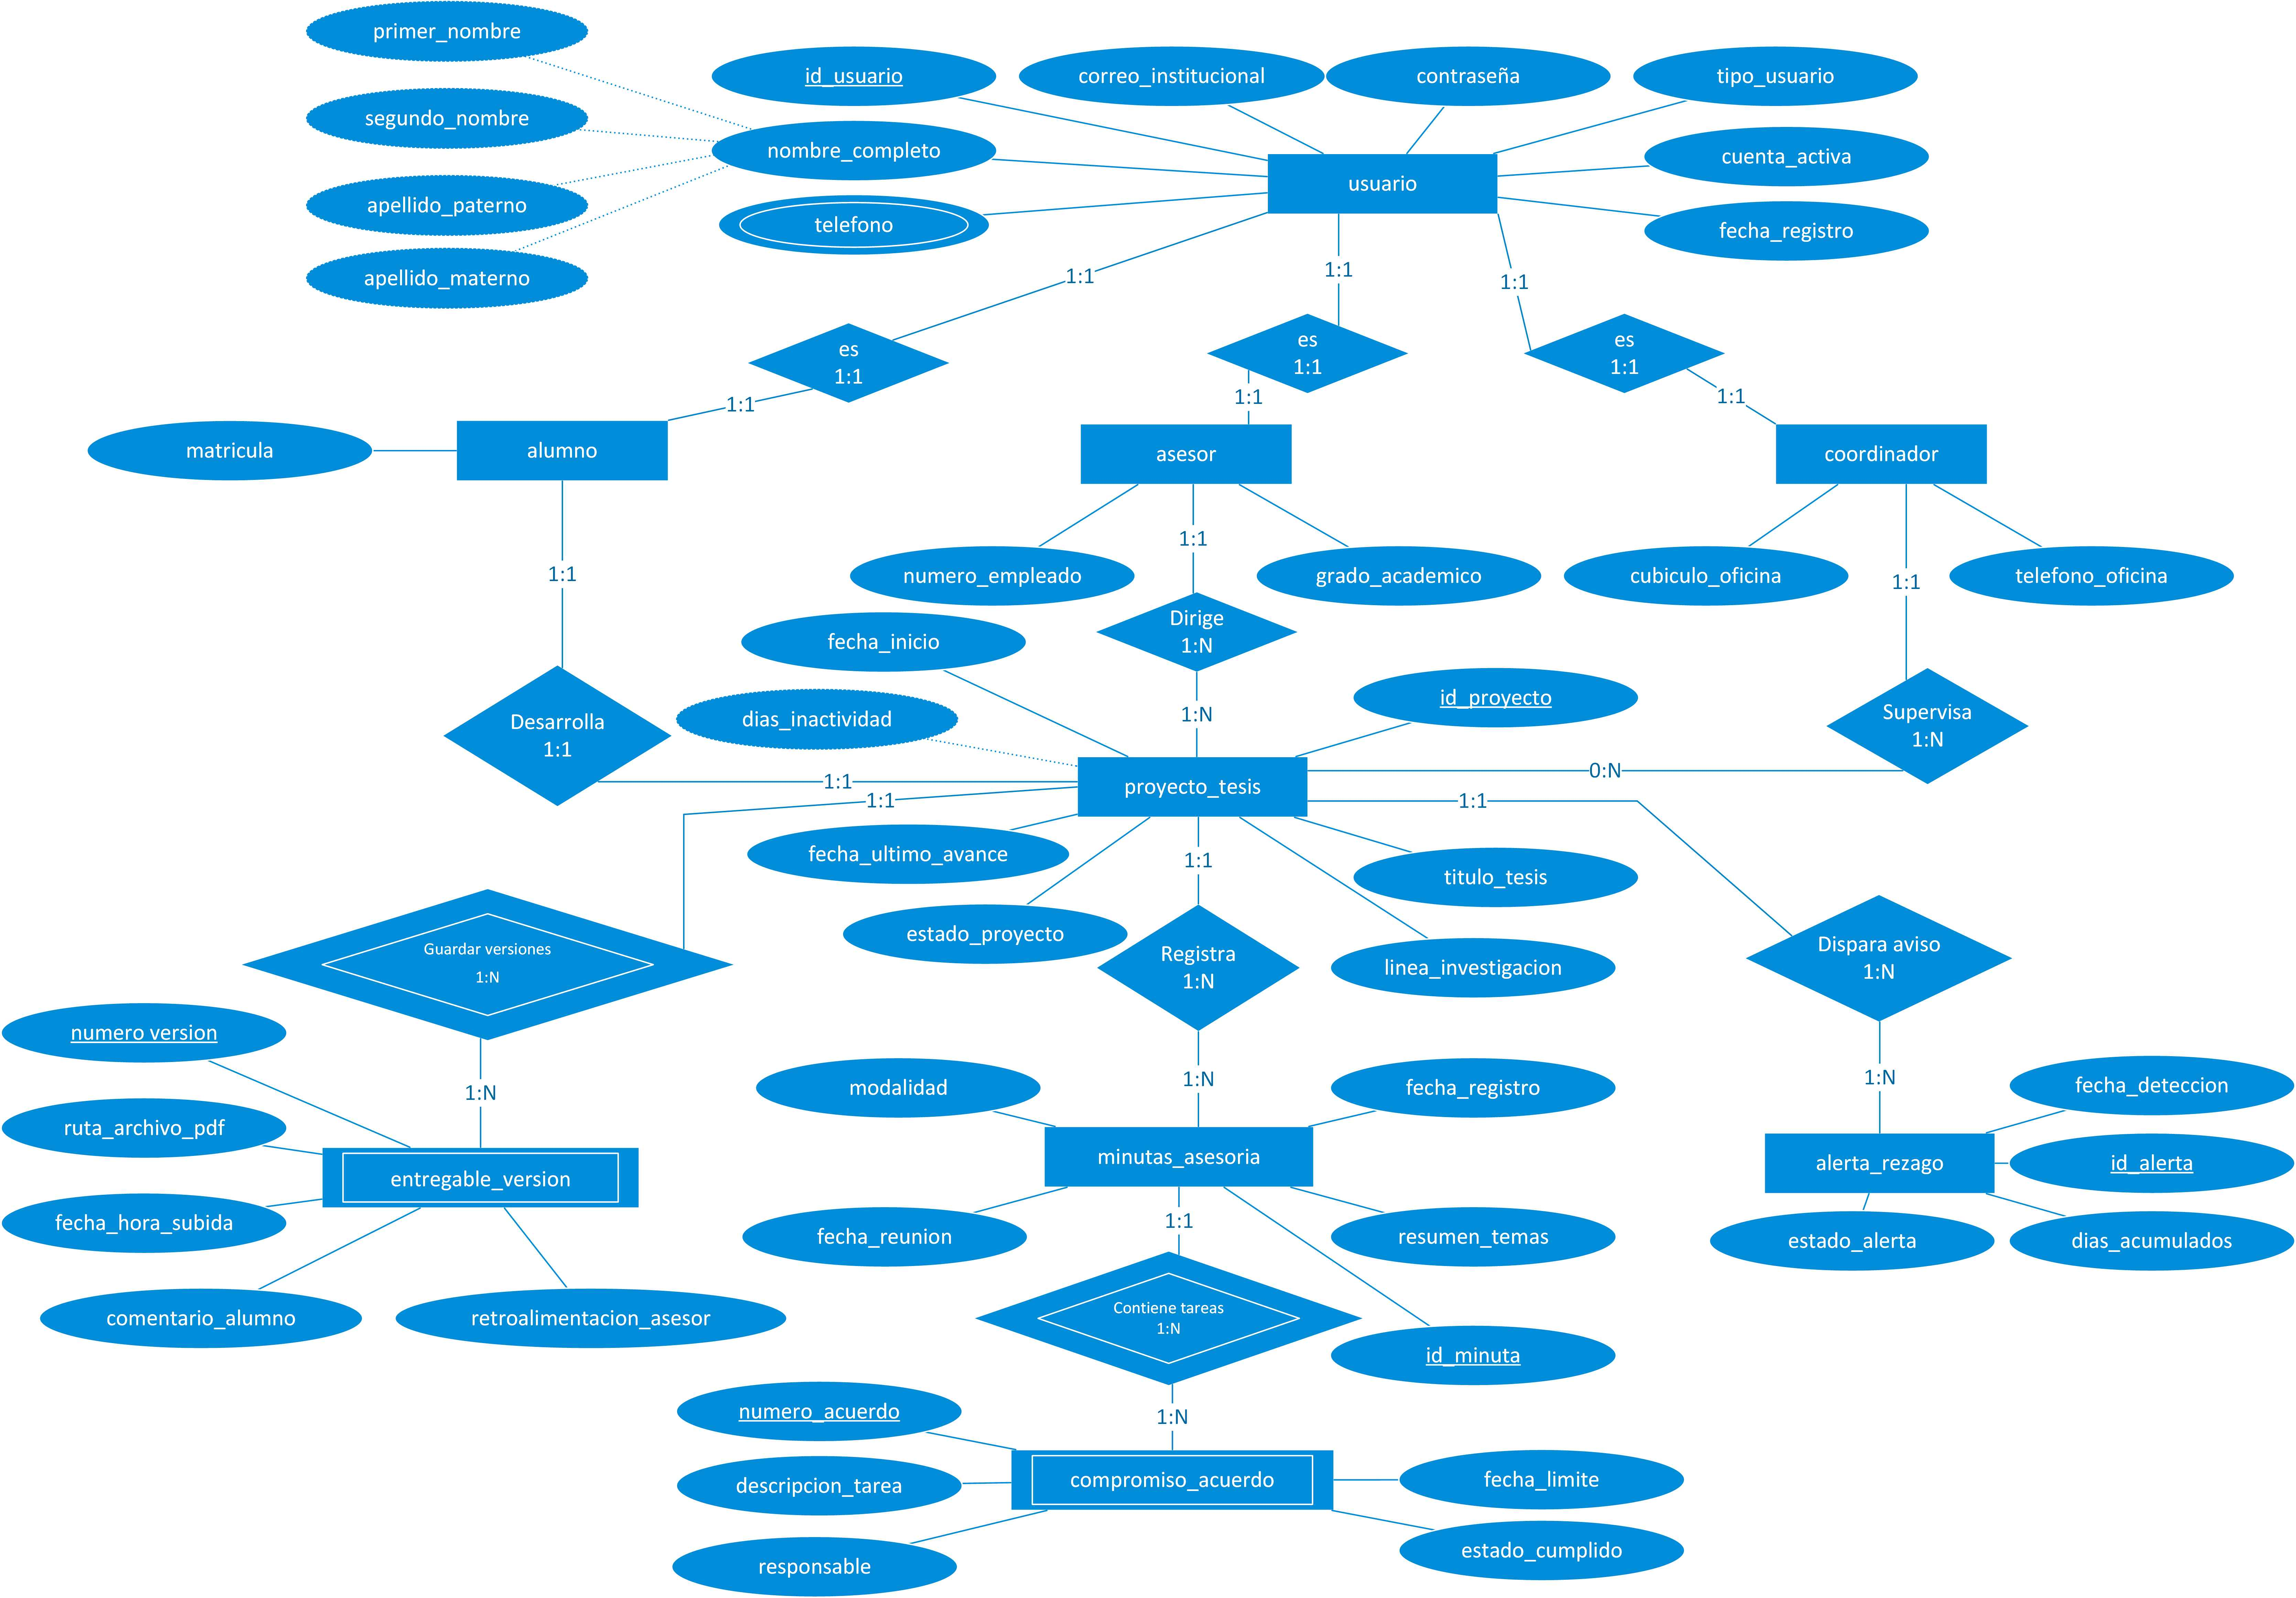
\includegraphics[width=1\linewidth]{assets/database/db-MER.jpg}
    \caption{Diagrama Entidad--Relación Extendido de la página web para seguimiento de tesis.}
    \label{fig:diagrama_eer}
\end{figure}